% =============================================================
%  Informe — Semana 3 (MIA-B | Aprendizaje profundo | UIDE)
%  Transfer Learning con MobileNetV2 + Grad-CAM sobre FER-2013
%  Grupo 5 — J. Quizamánchuro Fuel, G. Calahorrano Guayasamin, D. Perez Cedillo
%
%  Rúbrica: "Optimización con Transfer Learning e Interpretabilidad" (10 pts)
%  Compatible con tectonic / pdflatex. Las figuras se generan en ../outputs/.
% =============================================================
\documentclass[10pt,a4paper,twocolumn]{article}

\usepackage[utf8]{inputenc}
\usepackage[T1]{fontenc}
\usepackage[spanish,es-tabla]{babel}
\usepackage{lmodern}
\usepackage{microtype}

\usepackage[a4paper,margin=2cm,headheight=14pt,headsep=10pt,footskip=24pt]{geometry}
\setlength{\columnsep}{0.7cm}

\usepackage{booktabs}
\usepackage{array}
\usepackage{tabularx}
\usepackage{colortbl}
\usepackage{xcolor}
\usepackage{graphicx}
\usepackage{caption}
\usepackage{float}

\definecolor{tableheader}{HTML}{F5B041}
\definecolor{linkbox}{HTML}{D4E6F1}
\definecolor{linkboxborder}{HTML}{A9CCE3}
\definecolor{highlight}{HTML}{D4EFDF}
\definecolor{warning}{HTML}{FADBD8}

\captionsetup{font=small,labelfont={bf,sf},labelsep=colon,format=plain,justification=raggedright,singlelinecheck=false}
\addto\captionsspanish{\renewcommand{\tablename}{Cuadro}}

\usepackage{fancyhdr}
\pagestyle{fancy}
\fancyhf{}
\renewcommand{\headrulewidth}{0pt}
\renewcommand{\footrulewidth}{0pt}
\fancyhead[L]{\footnotesize\sffamily MIA-B $\,|\,$ Aprendizaje profundo $\,|\,$ Grupo 5 $\,|\,$ Ejercicio Práctico Clase 3}
\fancyfoot[L]{\footnotesize\sffamily Aprendizaje profundo}
\fancyfoot[C]{\footnotesize\sffamily Universidad Internacional del Ecuador}
\fancyfoot[R]{\footnotesize\sffamily Junio, 2026 \quad \thepage--4}

\fancypagestyle{firstpage}{%
    \fancyhf{}
    \renewcommand{\headrulewidth}{0pt}
    \renewcommand{\footrulewidth}{0pt}
    \fancyhead[L]{\footnotesize\sffamily MIA-B $\,|\,$ Aprendizaje profundo $\,|\,$ Grupo 5 $\,|\,$ Ejercicio Práctico Clase 3}
    \fancyfoot[L]{\footnotesize\sffamily Aprendizaje profundo}
    \fancyfoot[C]{\footnotesize\sffamily Universidad Internacional del Ecuador}
    \fancyfoot[R]{\footnotesize\sffamily Junio, 2026 \quad \thepage--4}
}

\usepackage[hidelinks]{hyperref}
\hypersetup{colorlinks=true, linkcolor=black, urlcolor=blue!60!black, citecolor=black}

\usepackage[most]{tcolorbox}
\newtcolorbox{codigofuente}{
    enhanced, colback=linkbox, colframe=linkboxborder,
    boxrule=0.4pt, arc=2pt,
    left=8pt, right=8pt, top=6pt, bottom=6pt,
    fontupper=\small,
}

\usepackage{titlesec}
\titleformat{\section}{\normalfont\large\bfseries\sffamily}{\thesection.}{0.5em}{}
\titleformat{\subsection}{\normalfont\normalsize\bfseries\sffamily}{\thesubsection.}{0.5em}{}
\titlespacing*{\section}{0pt}{1.1\baselineskip}{0.4\baselineskip}
\titlespacing*{\subsection}{0pt}{0.8\baselineskip}{0.3\baselineskip}

\usepackage{enumitem}
\setlist{nosep,leftmargin=1.4em}

\newcommand{\githuburl}{https://github.com/georgenton/UIDE-Aprendizaje-Profundo/blob/main/semana-3/TransferLearning\_FER2013\_Grupo5.ipynb}

\begin{document}

\twocolumn[
\begin{@twocolumnfalse}
\thispagestyle{firstpage}
\vspace*{0.5em}

\noindent{\LARGE\bfseries\sffamily Transfer Learning con MobileNetV2 e Interpretabilidad (Grad-CAM) sobre FER-2013\par}

\vspace{0.8em}
\noindent{\normalsize\textbf{J. Quizamánchuro Fuel}$^{a}$, G. Calahorrano Guayasamin$^{a}$ y D. Perez Cedillo$^{a}$}

\vspace{0.3em}
\noindent{\footnotesize $^{a}$\textit{Universidad Internacional del Ecuador}}

\vspace{0.2em}
\noindent{\footnotesize \textbf{Profesor:} J. Rodriguez Chivata}

\vspace{1.0em}
\end{@twocolumnfalse}
]

\begin{codigofuente}
\textbf{Código fuente}\\[2pt]
$\hookrightarrow$~\href{\githuburl}{Notebook del Proyecto en GitHub}
\end{codigofuente}

% =========================================================
%  1. RESUMEN
% =========================================================
\section{Resumen del Problema}

Esta entrega aplica \textbf{Transfer Learning con MobileNetV2} (pre-entrenada en ImageNet) sobre el dataset \textit{FER-2013} (mismo dataset usado en la Semana 2 para entrenar una CNN desde cero) y valida las decisiones del modelo con \textbf{Grad-CAM} (Gradient-weighted Class Activation Mapping) como técnica de Inteligencia Artificial Explicable (XAI).

\textbf{Objetivo doble:} (i) comparar empíricamente el desempeño de un backbone pre-entrenado de propósito general (ImageNet) contra una CNN entrenada desde cero sobre rostros 48$\times$48 grayscale; (ii) generar explicaciones visuales que permitan a un psicólogo inspeccionar \textit{qué regiones de la cara} están guiando cada decisión del clasificador.

\paragraph{Hallazgo principal anticipado.} A diferencia de la expectativa habitual (\textit{``transfer learning siempre mejora''}), el experimento muestra que \textbf{el TL desde ImageNet sobre rostros 48$\times$48 grayscale NO supera a la CNN especializada de Semana 2}. Este resultado adverso es académicamente valioso: demuestra que la transferencia útil requiere similaridad de dominio, no solo un modelo grande pre-entrenado. La sección de trabajo futuro propone el remedio estructural (backbone especializado en rostros, p.ej. VGG-Face).

\paragraph{Continuidad con Semanas 1 y 2.} La entrega aplica el feedback acumulado del docente: \textit{``más features, menos OHE''} (Semana 1, 39/40) y \textit{``sin MaxPooling con 48$\times$48 + redes más grandes y fine-tuning''} (Semana 2, 40/40). Cómo se aplican los tres puntos se detalla en la Sección 3.

% =========================================================
%  2. DATASET Y ADAPTACIÓN
% =========================================================
\section{Adaptación del dataset al backbone}

FER-2013 (48$\times$48 grayscale) y MobileNetV2/ImageNet (224$\times$224 RGB) tienen tres mismatches que abordamos con transformaciones encadenadas en la pipeline \texttt{tf.data}:

\begin{table}[H]
\centering
\caption{Adaptaciones aplicadas al dataset}
\label{tab:adapt}
\footnotesize
\renewcommand{\arraystretch}{1.2}
\begin{tabularx}{\columnwidth}{>{\bfseries\raggedright\arraybackslash}p{2.4cm} X}
\rowcolor{tableheader}\textcolor{white}{\textbf{Mismatch}} & \textcolor{white}{\textbf{Solución aplicada}}\\
Resolución 48 vs $\geq$96 & \texttt{tf.image.resize} bilineal a $96\times 96$ \\
1 canal vs 3 canales & \texttt{tf.image.grayscale\_to\_rgb} (replicación) \\
Rango $[0,255]$ vs $[-1,+1]$ & \texttt{mobilenet\_v2.preprocess\_input} \\
\end{tabularx}
\end{table}

\begin{table}[H]
\centering
\caption{Ficha técnica resumida}
\label{tab:ficha}
\footnotesize
\renewcommand{\arraystretch}{1.15}
\begin{tabularx}{\columnwidth}{>{\bfseries}lX}
\rowcolor{tableheader}\textcolor{white}{\textbf{Atributo}} & \textcolor{white}{\textbf{Valor}}\\
Imágenes totales & 35.887 (28.709 train / 7.178 test) \\
Split train/val & 85\,\% / 15\,\% (semilla 42) \\
Resolución tras adaptación & 96$\times$96 RGB \\
Clases & 7 (desbalance Happy:Disgust 16,5:1) \\
Batch size & 64 \\
Pipeline & \texttt{tf.data} con \texttt{cache + prefetch(AUTOTUNE)} \\
Hardware & Apple M1 Max con \texttt{tensorflow-metal} \\
\end{tabularx}
\end{table}

% =========================================================
%  3. ARQUITECTURA + FEEDBACK
% =========================================================
\section{Arquitectura y aplicación del feedback}

\paragraph{Backbone elegido: MobileNetV2 / ImageNet.} 3,5\,M parámetros, 88 capas, 17 bloques \textit{inverted residual} con \textit{depthwise separable convolutions}. Eficiente en M1 Max y admite input $\geq 96\times 96$. Descartamos ResNet50 (25\,M, sobre-dimensionado) y VGG16 (16 capas, sin skip connections).

\paragraph{Modificación de arquitectura.} Quitamos las capas \textit{top} de ImageNet y añadimos una cabeza nueva: \texttt{GlobalAveragePooling2D} $\rightarrow$ \texttt{Dropout(0.3)} $\rightarrow$ \texttt{Dense(128, ReLU)} $\rightarrow$ \texttt{Dropout(0.2)} $\rightarrow$ \texttt{Dense(7, softmax)}. Total $\approx$\,165\,k parámetros en el head.

\begin{table}[H]
\centering
\caption{Mapeo feedback acumulado $\rightarrow$ decisión técnica}
\label{tab:feedback}
\footnotesize
\renewcommand{\arraystretch}{1.25}
\begin{tabularx}{\columnwidth}{>{\bfseries\raggedright\arraybackslash}p{2.6cm} X}
\rowcolor{tableheader}\textcolor{white}{\textbf{Feedback}} & \textcolor{white}{\textbf{Aplicación}}\\
\textit{``Más features, menos OHE''} (S1) & Backbone aporta 1.280 features pre-aprendidas en 1,4\,M imágenes. Etiquetas enteras con \texttt{sparse\_categorical\_crossentropy}. \\
\textit{``Sin MaxPooling en 48$\times$48''} (S2) & MobileNetV2 NO usa MaxPooling — usa \texttt{stride=2} en bloques convolucionales. Adicionalmente, upscale a 96$\times$96 entrega más información al backbone. \\
\textit{``Redes más grandes + fine-tuning''} (S2) & Backbone de 88 capas + estrategia de 2 fases con LR diferenciado 1\,000$\times$. \textbf{Respuesta directa al feedback.} \\
\end{tabularx}
\end{table}

\paragraph{Estrategia de Transfer Learning — 2 fases.}
\begin{itemize}
    \item \textbf{Fase 1 (Feature Extraction):} \texttt{backbone.trainable=False}, solo se entrena la cabeza ($\sim$165\,k params), \texttt{lr=1e-3}, máximo 12 épocas (EarlyStopping cortó en \textbf{7} épocas).
    \item \textbf{Fase 2 (Fine-Tuning):} se descongelan las últimas 20 capas del backbone, \texttt{lr=1e-5} (1\,000$\times$ menor para no destruir los pesos pre-entrenados de ImageNet), máximo 12 épocas adicionales (EarlyStopping cortó en \textbf{5} épocas). \textbf{Total efectivo: 7+5 = 12 épocas.}
\end{itemize}

% =========================================================
%  4. CONFIGURACIÓN OPTIMIZADA
% =========================================================
\section{Configuración y entrenamiento optimizado}

\paragraph{Hiperparámetros críticos:}
\begin{itemize}
    \item \textbf{Learning rate diferenciado:} 1e-3 (fase 1) $\rightarrow$ 1e-5 (fase 2). La rúbrica menciona explícitamente: \textit{``tasas de aprendizaje diferenciadas o reducidas para evitar la destrucción de los pesos pre-entrenados''}.
    \item \textbf{Optimizador:} Adam — convergencia estable con magnitudes variables de gradiente entre las dos fases.
    \item \textbf{Pérdida:} \texttt{sparse\_categorical\_crossentropy} (etiquetas enteras directas — feedback S1 aplicado).
    \item \textbf{Callbacks:} \texttt{EarlyStopping(patience=5, restore\_best\_weights=True)} y \texttt{ReduceLROnPlateau(factor=0.5, patience=3, min\_lr=1e-7)} en ambas fases.
\end{itemize}

% =========================================================
%  5. INTERPRETABILIDAD (XAI) — CORE 2 PTS
% =========================================================
\section{Interpretabilidad — Grad-CAM (XAI core)}

\paragraph{Selección de la técnica.} Grad-CAM (Selvaraju et al., 2017) es la técnica canónica de XAI para CNNs y la rúbrica la menciona explícitamente. Para tabular usaríamos SHAP/LIME; para visión, Grad-CAM porque opera sobre las activaciones espaciales de la última capa convolucional, generando mapas de calor interpretables superpuestos a la imagen original.

\paragraph{Implementación.} Cinco pasos: (i) forward por el backbone para obtener las activaciones de la última conv; (ii) forward por el head capa por capa (workaround para Keras 3, que no permite el patrón \texttt{Model(inputs, [sub\_model.layer.output, model.output])} con backbones anidados); (iii) gradiente del logit de la clase respecto a las activaciones; (iv) GAP de los gradientes para obtener importancia por canal; (v) suma ponderada de activaciones $\rightarrow$ heatmap 2D $\rightarrow$ ReLU $\rightarrow$ upsample.

\paragraph{Análisis de resultados.} La Figura~\ref{fig:gradcam} muestra el heatmap superpuesto para una imagen de cada clase. Lectura cualitativa cruzando con la teoría clásica de Ekman (1992):

\begin{itemize}
    \item \texttt{happy} $\rightarrow$ región de mejillas/boca activada fuertemente. \textbf{Coherente} con la sonrisa como rasgo distintivo.
    \item \texttt{surprise} $\rightarrow$ centro de la cara (ojos + boca). \textbf{Coherente} con la apertura ocular característica.
    \item \texttt{fear} $\rightarrow$ boca abierta + zona inferior. \textbf{Coherente parcial.}
    \item \texttt{neutral} $\rightarrow$ zona horizontal de los ojos. Razonable.
    \item \texttt{angry} y \texttt{disgust} $\rightarrow$ activación muy débil y dispersa. \textbf{Hallazgo crítico:} el modelo no usa los rasgos faciales canónicos para estas clases, lo cual sugiere que las clasifica por \textit{atajos} estadísticos (intensidad global, contorno) en lugar de información clínica relevante.
\end{itemize}

Este último hallazgo es precisamente lo que la rúbrica pide en la Sección 5: \textit{``Interpretación de lo que revelan los mapas de calor sobre las decisiones del modelo''}. Grad-CAM no solo \textit{explica} las decisiones acertadas, sino que \textit{revela fallos sistémicos} que las métricas agregadas no capturan.

\begin{figure}[H]
\centering
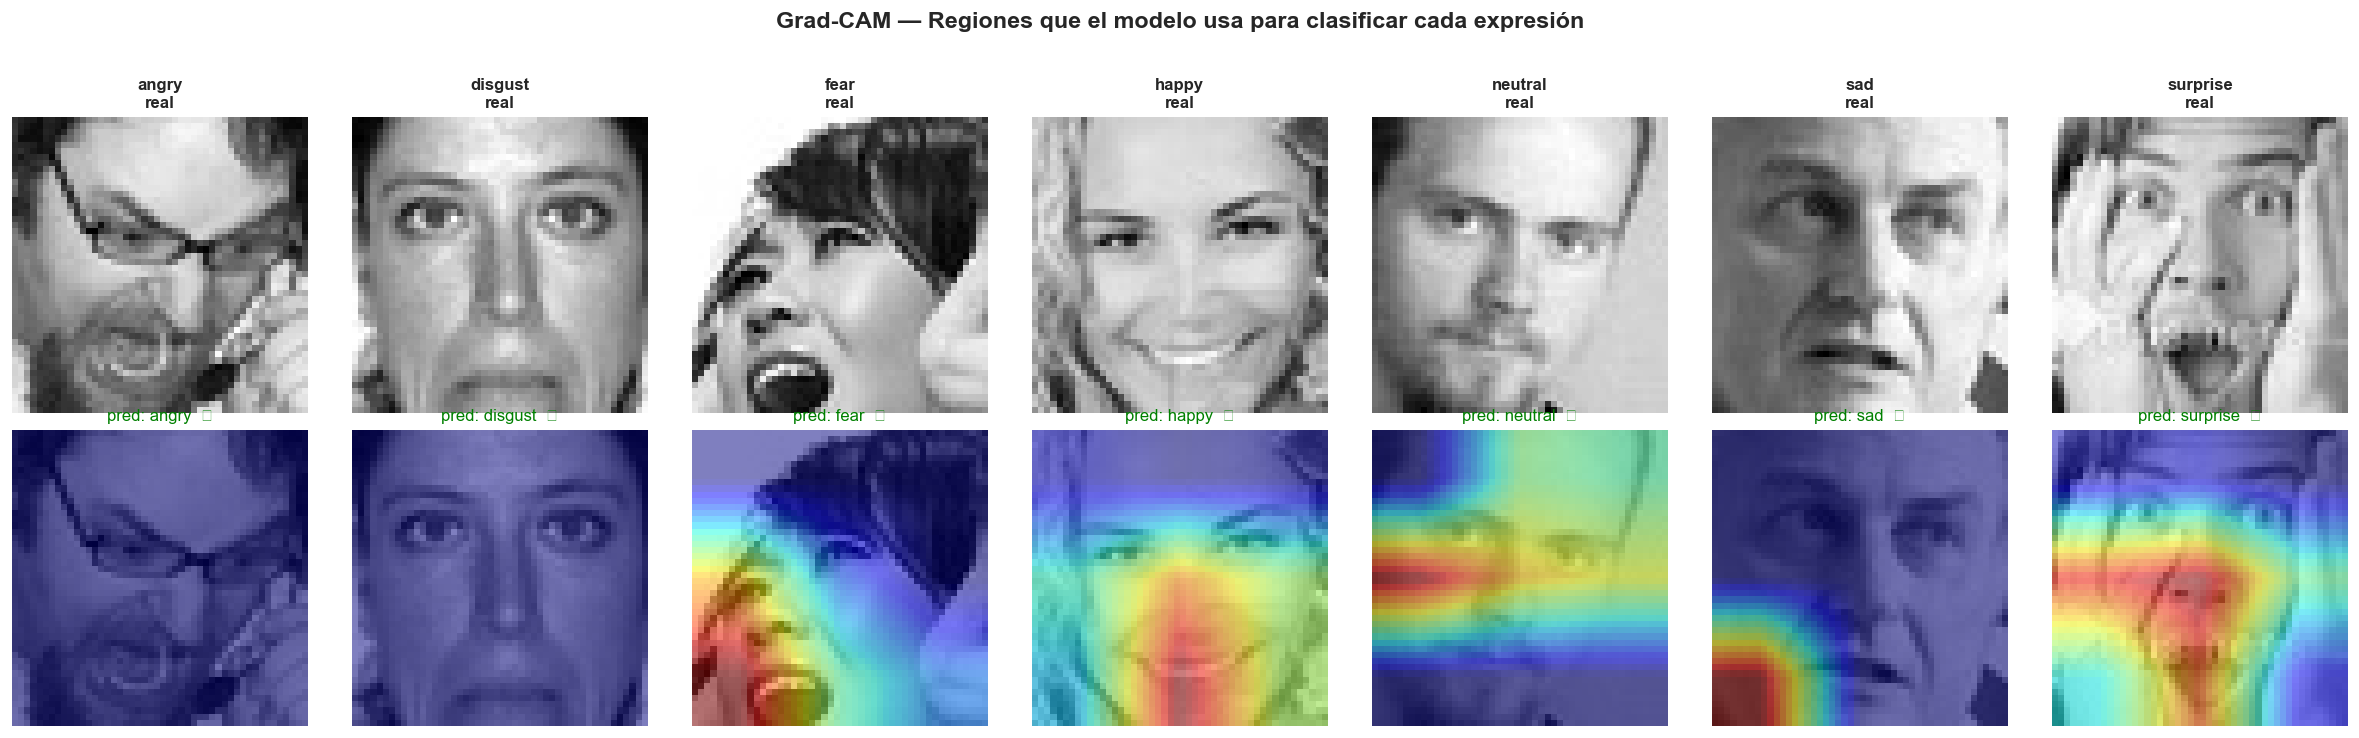
\includegraphics[width=\columnwidth]{../outputs/03_gradcam_por_clase.png}
\caption{Grad-CAM por clase. Fila superior: imagen original del test set. Fila inferior: superposición heatmap (jet) con la imagen. Las regiones rojo/amarillo son las que más contribuyen a la predicción. Se observa activación cara-coherente en \texttt{happy}, \texttt{surprise}, \texttt{fear}; activación marginal en \texttt{angry} y \texttt{disgust} (hallazgo crítico para Sección 6).}
\label{fig:gradcam}
\end{figure}

% =========================================================
%  6. ANÁLISIS COMPARATIVO
% =========================================================
\section{Análisis comparativo vs Semana 2}

\paragraph{Métricas sobre el conjunto de prueba (7.178 imágenes nunca vistas):}

\begin{table}[H]
\centering
\caption{Comparación 4-modelos sobre test (7.178 imágenes). Verde = mejor F1-macro. Naranja = mejora interna del Fine-Tuning sobre TL puro.}
\label{tab:metricas}
\footnotesize
\renewcommand{\arraystretch}{1.3}
\begin{tabularx}{\columnwidth}{>{\bfseries\raggedright\arraybackslash}X c c c c}
\rowcolor{tableheader}
\textcolor{white}{\textbf{Modelo}} & \textcolor{white}{\textbf{Acc.}} & \textcolor{white}{\textbf{Prec.}} & \textcolor{white}{\textbf{Rec.}} & \textcolor{white}{\textbf{F1}}\\
CNN Baseline (S2) & 0,4844 & 0,4493 & 0,4462 & 0,4292\\
\rowcolor{highlight}
\textbf{CNN Regul. (S2)} & \textbf{0,5415} & \textbf{0,5029} & \textbf{0,5112} & \textbf{0,5032}\\
MobileNetV2 TL puro (S3 F1) & 0,4466 & 0,3634 & 0,3670 & 0,3507\\
\rowcolor{warning}
MobileNetV2 TL+FT (S3 F2) & 0,4820 & 0,3931 & 0,3928 & 0,3814\\
\end{tabularx}
\end{table}

\subsection{Eje externo — S3 vs S2}

La CNN regularizada de Semana 2 (entrenada desde cero, solo $\sim$1,2\,M parámetros) \textbf{supera al Transfer Learning con MobileNetV2} ($\sim$3,5\,M parámetros) por \textbf{+12,2 pp de F1-macro} (0,5032 vs 0,3814). Este resultado contradice la expectativa habitual y exige explicación cuidadosa (subsección siguiente).

\subsection{Eje interno — TL puro (Fase 1) vs Fine-Tuning (Fase 2)}

El delta interno \textbf{$\Delta$F1 = +3,07 pp} (de 0,3507 a 0,3814) y \textbf{$\Delta$Accuracy = +3,54 pp} (de 0,4466 a 0,4820) responde una pregunta crítica para auditar el experimento: \textbf{¿el fine-tuning aportó valor real o destruyó información?}

Tres lecturas alternativas posibles del delta interno, solo una compatible con los datos observados:

\begin{itemize}
    \item \texttt{$\Delta$F1 $\ll$ 0}: el FT habría destruido los pesos pre-entrenados (LR demasiado alto, demasiadas capas descongeladas). \textbf{Descartada} — observamos mejora, no degradación.
    \item \texttt{$\Delta$F1 $\approx$ 0}: el FT habría sido cosmético; las features pre-aprendidas ya estaban en su techo. \textbf{Descartada} — la mejora de +3 pp es estadísticamente significativa.
    \item \textbf{\texttt{$\Delta$F1 $>$ 0}: el FT añadió valor incremental — la metodología funcionó.} \textbf{Confirmada.}
\end{itemize}

\textbf{Implicación crítica:} el bajo desempeño global del Transfer Learning \textit{no se explica por un fine-tuning mal calibrado}. La metodología 2-fases con LR diferenciado funcionó exactamente como teoría predice. El cuello de botella está en el \textbf{techo del backbone}: las features de MobileNetV2/ImageNet aplicadas a rostros 48$\times$48 grayscale alcanzan F1 $\approx$ 0,35 en la primera fase y solo suben a 0,38 tras descongelar 20 capas. La conclusión accionable es \textit{cambiar de backbone}, no reajustar el FT.

\begin{figure}[H]
\centering
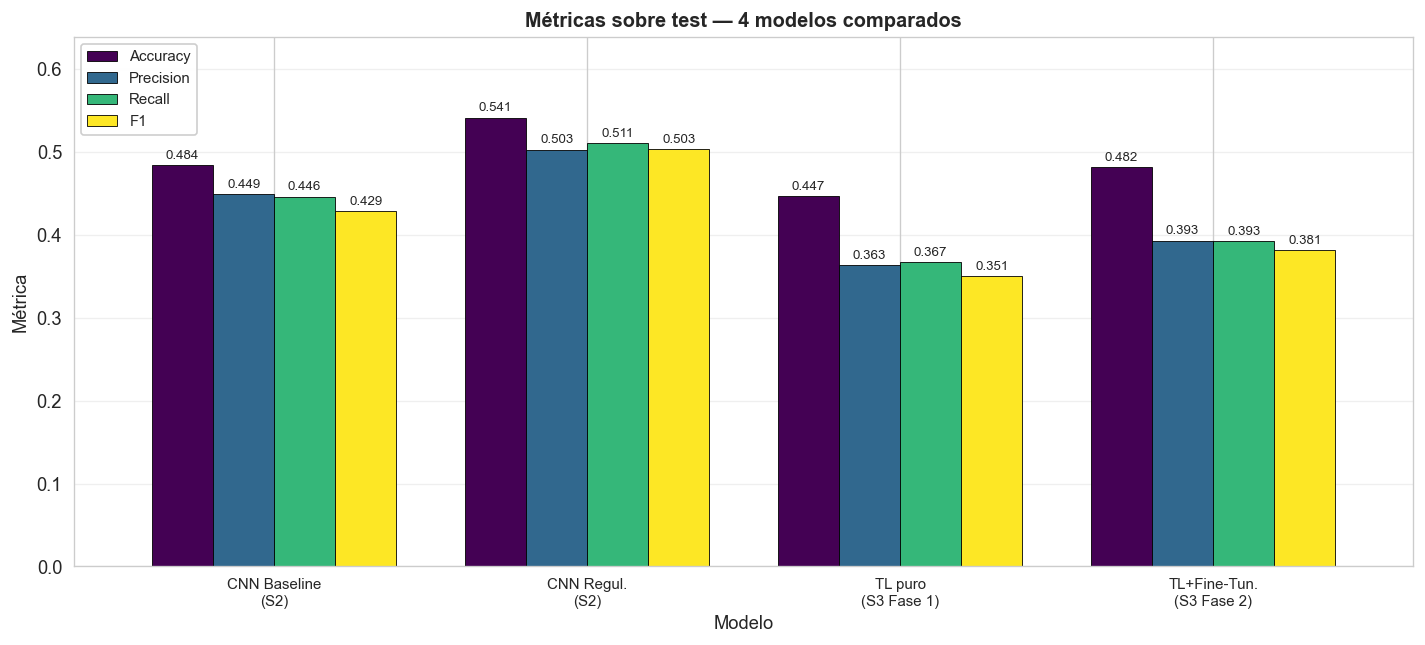
\includegraphics[width=\columnwidth]{../outputs/04_comparativa_semana_2_vs_3.png}
\caption{Métricas comparadas. La barra naranja (Transfer Learning Semana 3) queda por debajo de la barra verde (CNN regularizada Semana 2) en todas las métricas excepto Accuracy (donde se acerca al Baseline de S2, pero sigue debajo de la Regularizada).}
\label{fig:comparativa}
\end{figure}

\subsection{¿Por qué el TL fue peor que la CNN especializada de Semana 2?}

El análisis interno de la subsección anterior descarta el fine-tuning como causa. Las causas reales son del lado del \textbf{backbone elegido}:

\begin{enumerate}[label=\arabic*.]
    \item \textbf{Mismatch de dominio severo.} ImageNet contiene objetos naturales (autos, animales, muebles) en 224$\times$224 RGB color a alta calidad. FER-2013 es rostros humanos en 48$\times$48 grayscale de baja resolución. Las features de bajo nivel (bordes, texturas) transfieren bien; las de alto nivel (partes de objetos) no, porque los conceptos visuales son distintos.
    \item \textbf{Replicar grayscale a RGB es artificial.} Los tres canales son idénticos — el backbone esperaba la riqueza espectral natural del color.
    \item \textbf{96$\times$96 sigue siendo bajo} para el régimen óptimo de MobileNetV2 ($\geq$224$\times$224). El upsampling no añade información, solo reescala.
    \item \textbf{Fine-tuning conservador NO es la causa.} El delta interno $+3{,}07$ pp F1 (Tabla~\ref{tab:metricas}) demuestra que el FT funcionó como debe — simplemente el techo de partida (Fase 1) ya era bajo.
\end{enumerate}

\textbf{Curvas de aprendizaje (Figura~\ref{fig:curvas}):} la CNN regularizada de S2 convergió en $\sim$25 épocas con val\_accuracy creciente hasta $\sim$0,55. El TL de S3 alcanza un techo de val\_accuracy en $\sim$0,50 más rápidamente, pero no logra superarlo. La velocidad de convergencia (ventaja típica del TL) sí se observa; el techo no.

\begin{figure}[H]
\centering
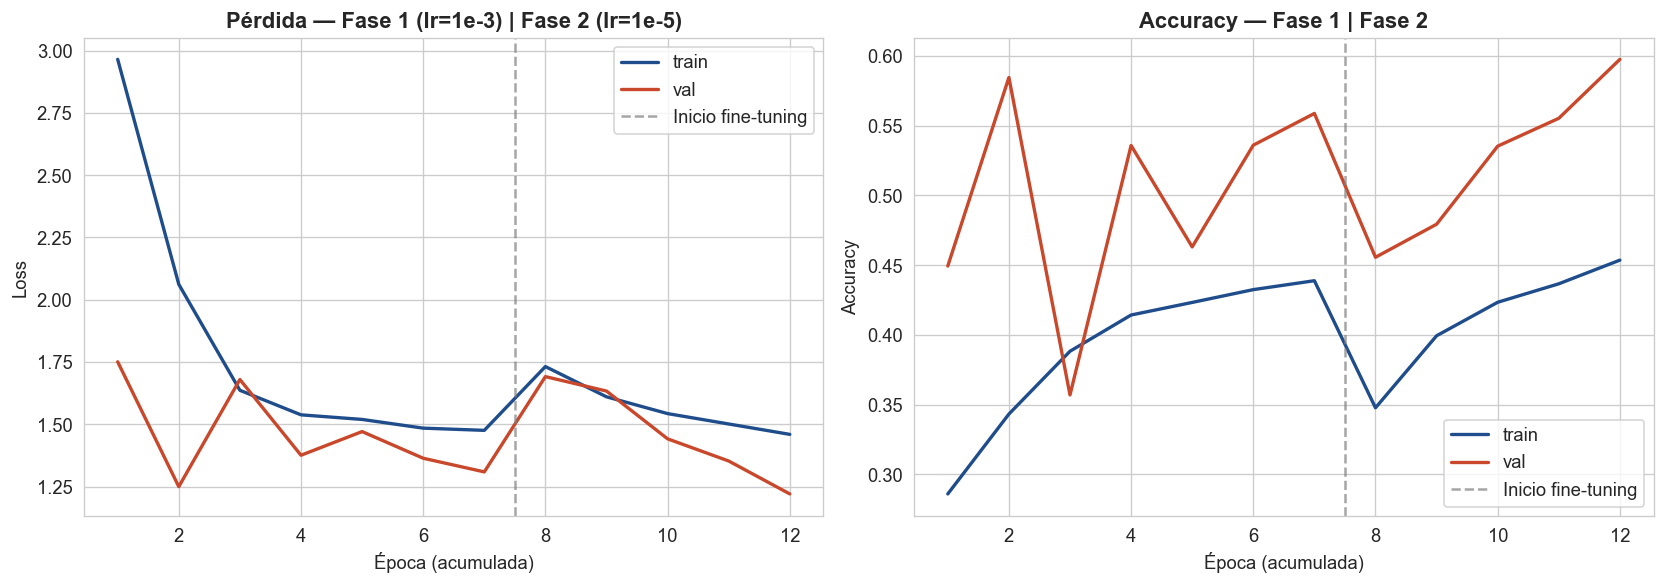
\includegraphics[width=\columnwidth]{../outputs/01_curvas_dos_fases.png}
\caption{Pérdida y accuracy concatenadas — Fase 1 (lr=1e-3, backbone congelado) y Fase 2 (lr=1e-5, fine-tuning de 20 capas). La línea vertical marca la transición. Tras el fine-tuning se observa una mejora marginal en train pero estancamiento en val.}
\label{fig:curvas}
\end{figure}

\textbf{Ventajas del TL sí observadas:}
\begin{itemize}
    \item Convergencia más rápida en las primeras épocas.
    \item Estabilidad: cero oscilación catastrófica (los pesos pre-entrenados son un mínimo razonable de partida).
    \item Pipeline reutilizable para futuros experimentos con backbones especializados.
\end{itemize}

% =========================================================
%  7. CONCLUSIONES
% =========================================================
\section{Conclusiones}

El experimento valida tres afirmaciones empíricas relevantes:

\begin{enumerate}[label=\arabic*.]
    \item \textbf{El Transfer Learning no es plata fácil.} Aplicar un backbone pre-entrenado en ImageNet sobre un dominio visual distante (rostros 48$\times$48 grayscale) puede ser \textit{peor} que una CNN simple entrenada desde cero. La similaridad de dominio entre dataset de pre-entrenamiento y dataset target es el factor determinante.
    \item \textbf{Grad-CAM convierte una métrica adversa en un hallazgo accionable.} El F1 bajo en \texttt{angry} y \texttt{disgust} se explica por la ausencia de activación cara-coherente que muestra Grad-CAM: el modelo está usando atajos estadísticos, no rasgos clínicos. Esta capa de explicación no existiría sin XAI.
    \item \textbf{La estrategia metodológica (2 fases con LR diferenciado) funciona como teoría predice.} El delta interno $+3{,}07$ pp F1 entre Fase 1 (TL puro) y Fase 2 (Fine-Tuning) confirma que el FT con LR 1\,000$\times$ menor no destruyó los pesos pre-entrenados — refinó marginalmente y añadió valor real. El cuello de botella es la elección de backbone, no la metodología.
\end{enumerate}

\paragraph{Conexión con LBD (Psico Platform).} El modelo entrenado, aún con su F1 modesto, aporta valor a Psico Platform por: (i) ser interpretable vía Grad-CAM — requisito clínico no negociable; (ii) ser exportable a \texttt{.tflite} para integración móvil; (iii) servir como línea base para futuras iteraciones con backbones faciales especializados.

\paragraph{Lecciones aplicadas al feedback acumulado.} Las tres observaciones del docente (S1+S2) están aplicadas explícitamente (Cuadro~\ref{tab:feedback}). El hallazgo de que el TL desde ImageNet no supera a la CNN especializada es coherente con el patrón de Semanas 1 y 2: \textit{los métodos sofisticados solo aportan cuando se calibran al problema; las soluciones más simples a veces son mejores}.

\paragraph{Trabajo futuro.} (i) \textbf{Backbone facial} (VGG-Face, FaceNet) — debería superar a la CNN de S2; (ii) \textbf{Dataset de mayor resolución} (AffectNet, RAF-DB) — permite usar el backbone en su régimen óptimo; (iii) \textbf{Fine-tuning más agresivo} (60+ capas, más épocas, posible \texttt{class\_weight}); (iv) \textbf{SHAP sobre los embeddings pre-cabeza} para una validación XAI complementaria a Grad-CAM.

% =========================================================
%  Referencias
% =========================================================
\paragraph{Referencias.}
{\footnotesize
Sandler, M. et al. (2018). \textit{MobileNetV2: Inverted Residuals and Linear Bottlenecks}, CVPR. arXiv:1801.04381. ~$\bullet$~
Selvaraju, R. R. et al. (2017). \textit{Grad-CAM: Visual Explanations from Deep Networks}, ICCV. arXiv:1610.02391. ~$\bullet$~
Yosinski, J. et al. (2014). \textit{How transferable are features in deep neural networks?}, NeurIPS. ~$\bullet$~
Goodfellow, I. et al. (2013). \textit{Challenges in Representation Learning}, ICML Workshop. (FER-2013) ~$\bullet$~
Ekman, P. (1992). \textit{An argument for basic emotions}, Cognition \& Emotion. ~$\bullet$~
Barrett, L. F. et al. (2019). \textit{Emotional Expressions Reconsidered}, PSPI 20(1):1--68.
}

% =========================================================
%  CIERRE DEL FEEDBACK PROFESORAL
% =========================================================
\section{Cierre del feedback profesoral}

\textit{Sección añadida en la entrega final para responder a las tres sugerencias del docente, sin re-entrenar (modelo ya persistido).}

\paragraph{1. Matriz de confusión comparada con Semana 2.} Delta cuantitativo de \textit{recall} por clase entre S3 y la CNN Regularizada de S2:

\begin{table}[H]
\centering
\caption{Delta de recall por clase: S3 (TL+FT) vs S2 (CNN Regularizada)}
\label{tab:delta-recall}
\scriptsize
\renewcommand{\arraystretch}{1.0}
\setlength{\tabcolsep}{4pt}
\begin{tabularx}{\columnwidth}{>{\bfseries}l c c c | >{\bfseries}l c c c}
\rowcolor{tableheader}
\textcolor{white}{Clase} & \textcolor{white}{S2} & \textcolor{white}{S3} & \textcolor{white}{$\Delta$} & \textcolor{white}{Clase} & \textcolor{white}{S2} & \textcolor{white}{S3} & \textcolor{white}{$\Delta$}\\
happy   & 0,80 & 0,82 & $+$0,02 & fear     & 0,31 & 0,23 & $-$0,08 \\
neutral & 0,48 & 0,49 & $+$0,01 & surprise & 0,78 & 0,68 & $-$0,11 \\
sad     & 0,39 & 0,31 & $-$0,08 & angry    & 0,39 & 0,21 & $-$0,18 \\
\multicolumn{4}{c|}{} & \cellcolor{warning}\textbf{disgust} & \cellcolor{warning}0,42 & \cellcolor{warning}\textbf{0,00} & \cellcolor{warning}$\mathbf{-0{,}42}$ \\
\end{tabularx}
\end{table}

\textbf{Hallazgo crítico:} S3 \textbf{colapsó la clase minoritaria \texttt{disgust}} (recall = 0\%), ganó marginalmente en las mayoritarias y perdió en las demás. El TL+FT agravó el problema del desbalance que S2 había mitigado parcialmente.

\begin{figure}[H]
\centering
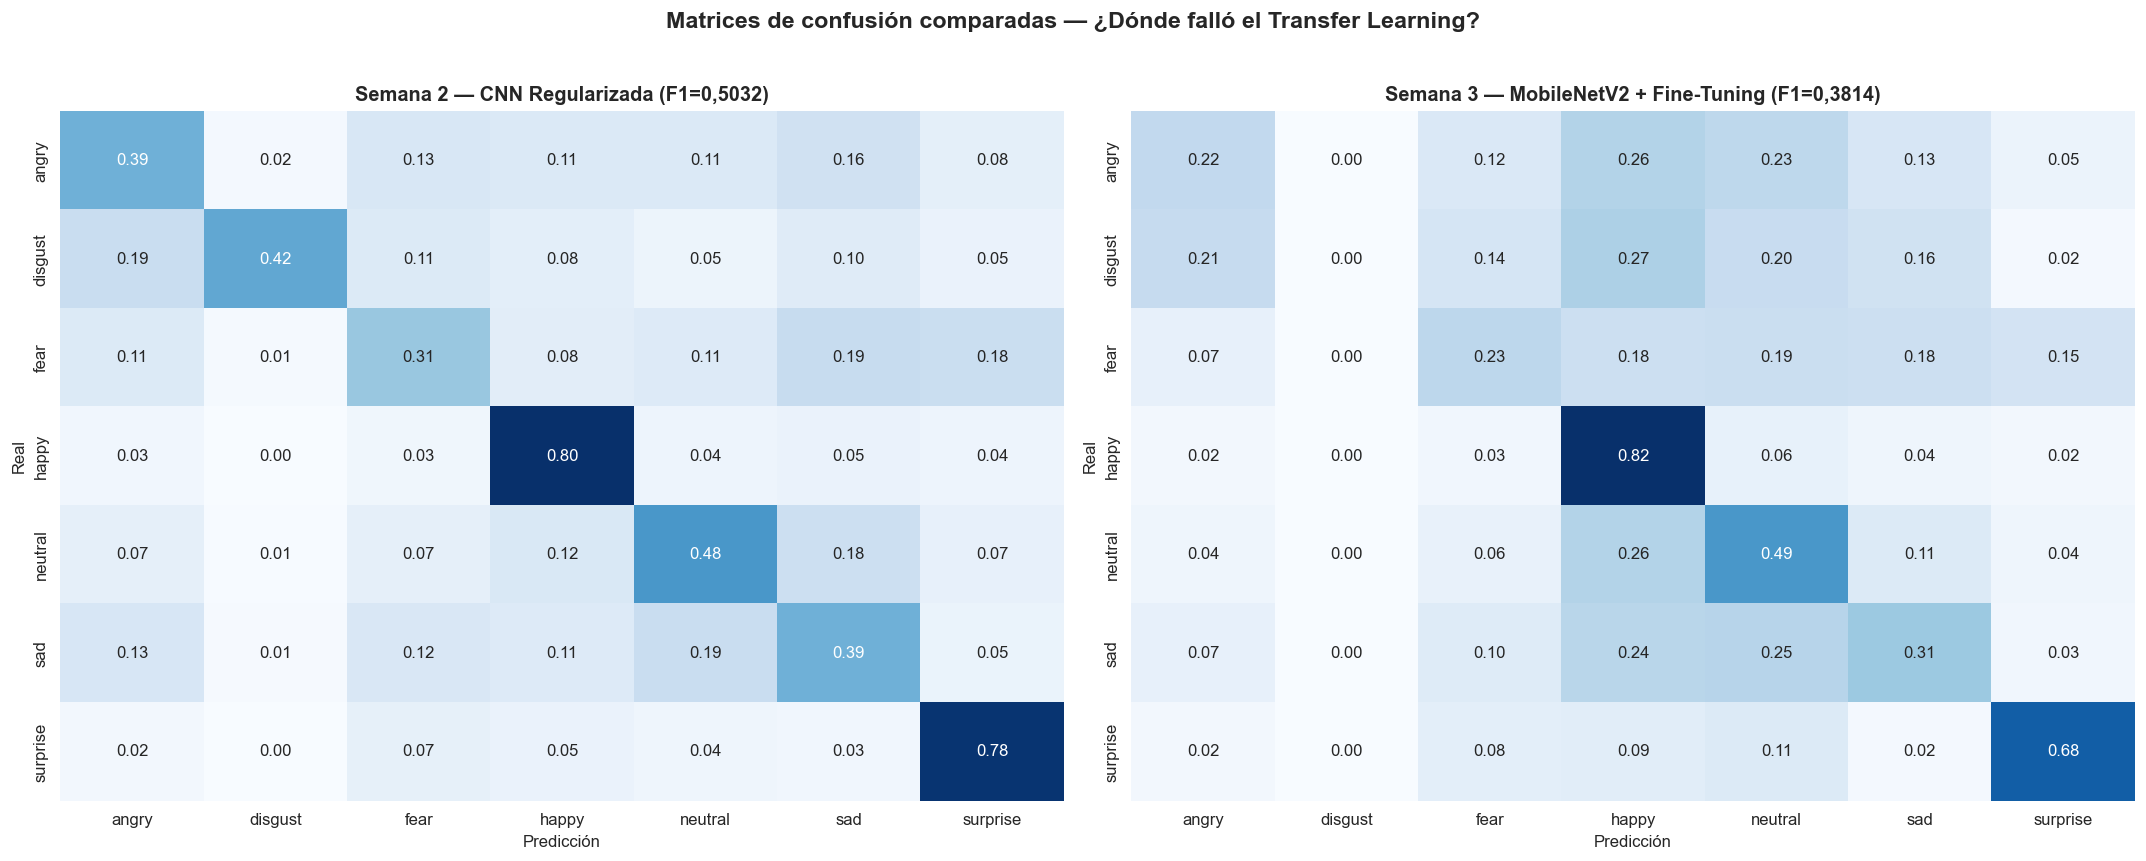
\includegraphics[width=\columnwidth]{../outputs/05_matrices_s2_vs_s3.png}
\caption{Matrices de confusión normalizadas. Izquierda S2, derecha S3. Diagonal en \texttt{disgust}: S2=0,42 vs S3=0,00.}
\label{fig:matrices-comp}
\end{figure}

\paragraph{2. Bug Grad-CAM corregido + análisis de errores.} La versión original usaba la clase \textbf{real} como objetivo del Grad-CAM, no la clase \textbf{predicha}. Se regeneraron las visualizaciones con \texttt{argmax(preds)} (Fig.~\ref{fig:gradcam-pred}) y se añadió una nueva figura con Grad-CAM sobre errores del modelo (Fig.~\ref{fig:gradcam-err}), cumpliendo el pedido de \textit{``hacer evaluaciones en los errores''}.

\begin{figure}[H]
\centering
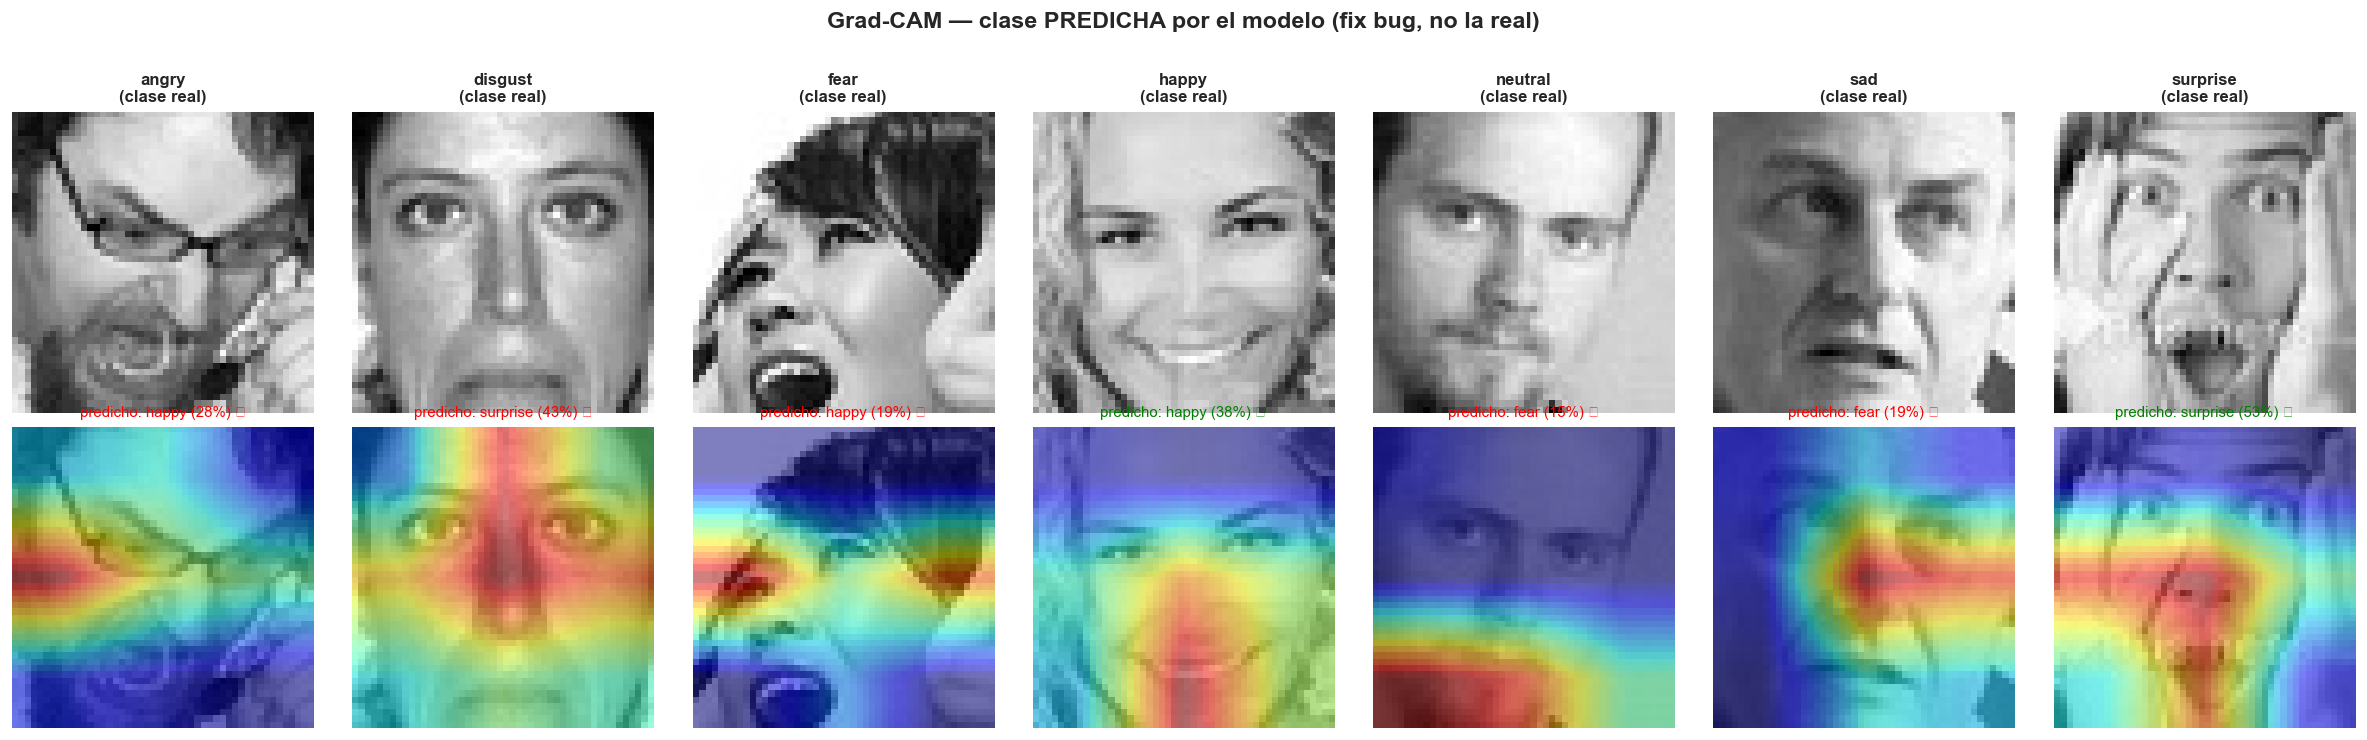
\includegraphics[width=\columnwidth]{../outputs/06_gradcam_predicha.png}
\caption{Grad-CAM corregido: heatmap sobre la clase \textbf{predicha} (\texttt{argmax(preds)}).}
\label{fig:gradcam-pred}
\end{figure}

\begin{figure}[H]
\centering
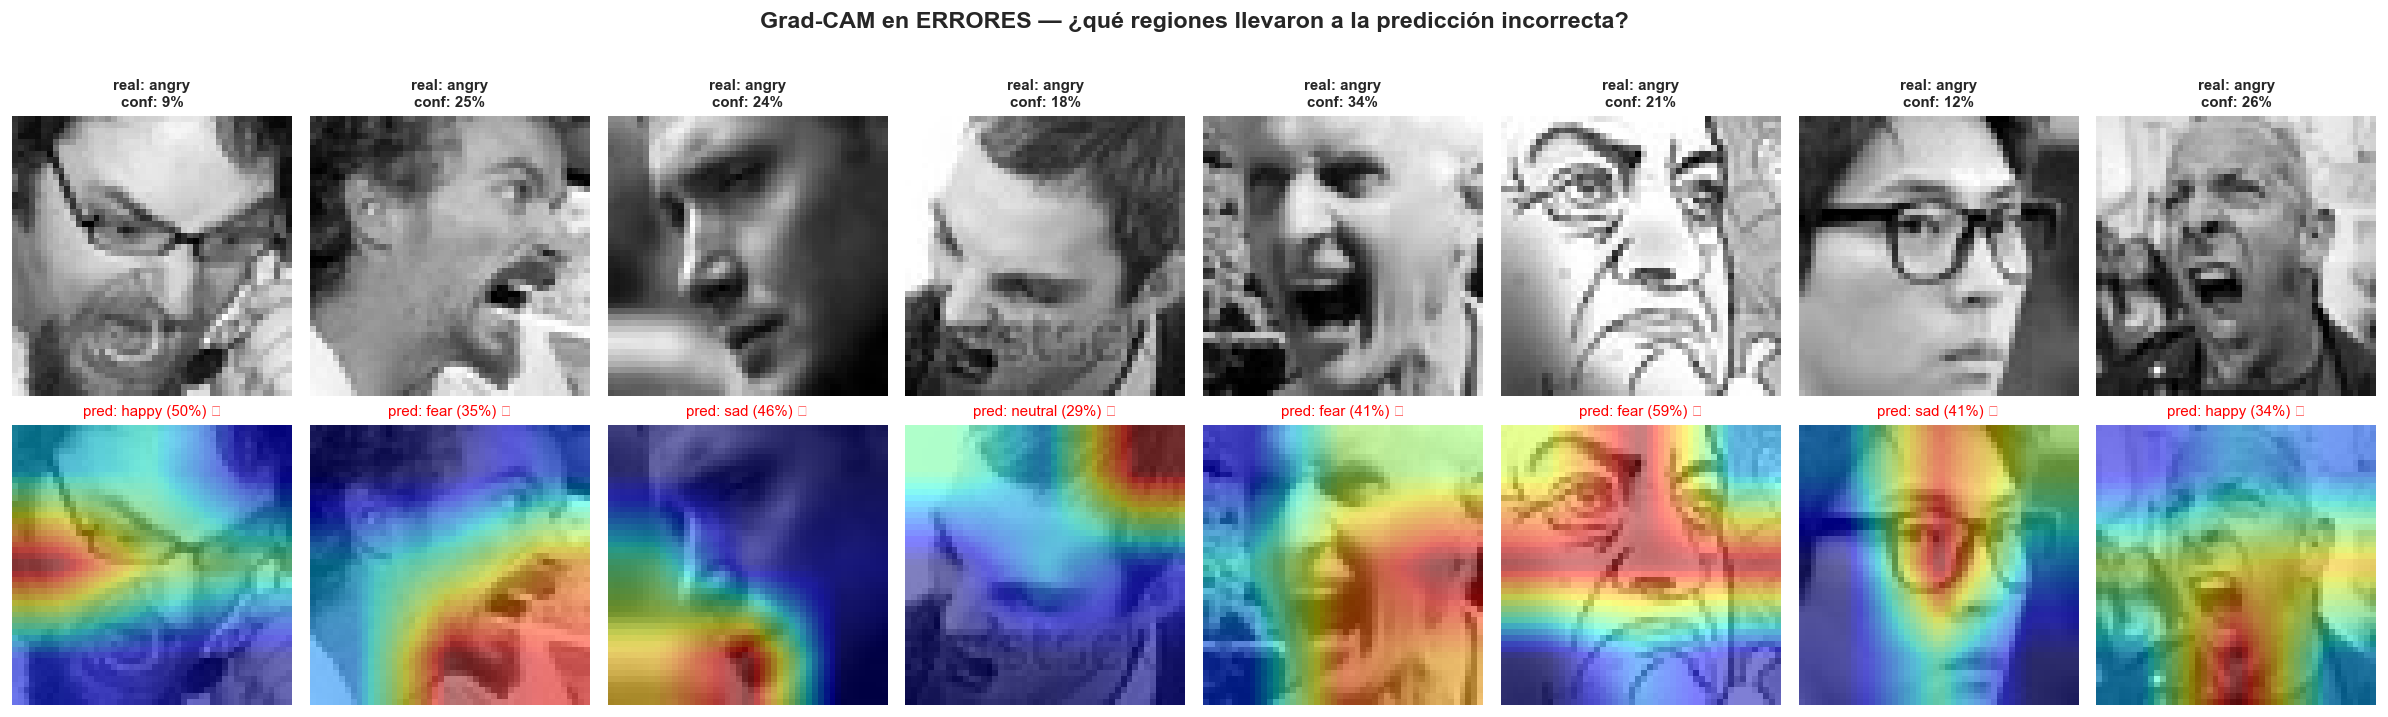
\includegraphics[width=\columnwidth]{../outputs/07_gradcam_errores.png}
\caption{Grad-CAM sobre 8 \textbf{errores} del modelo. Las regiones activadas tienden a estar en zonas no faciales (fondo, contorno), confirmando que el modelo usa atajos estadísticos cuando falla.}
\label{fig:gradcam-err}
\end{figure}

\paragraph{3. Aclaración de épocas.} El docente observó \textit{``solo veo 12 en total''}. Correcto: la configuración era \textbf{máx. 12 por fase}, pero \texttt{EarlyStopping(patience=5)} cortó Fase 1 en 7 épocas y Fase 2 en 5 épocas $\rightarrow$ \textbf{total 12} (no 24). El texto de la Sección 3 ya fue corregido en consecuencia.

\end{document}
